\documentclass{article}

% r47b: without an explicit font encoding, tectonic compiles under TU and every Times shape
% requested by the mandated `times' package is undefined (ptm/m/n, ptm/b/n, ptm/m/it, ptm/m/sc,
% pcr/m/n), so the whole manuscript silently fell back to Latin Modern Regular: \textbf and
% \emph printed at regular weight and upright. T1 restores real bold/italic/small-caps Times.
% The official iclr2026_conference.sty/.bst are untouched.
\usepackage[T1]{fontenc}
\usepackage{iclr2026_conference,times}
\usepackage{amsmath,amssymb,booktabs,float,graphicx,microtype}
\usepackage{tabularx}
\usepackage[hidelinks]{hyperref}
% r47 layout compaction: typography only, no claim, number, table row, figure panel or
% limitation is removed to fit the page budget. The official iclr2026_conference.sty is
% untouched; these are document-level lengths and a caption font choice.
\usepackage[font=small,skip=6pt]{caption}
\setlength{\textfloatsep}{12pt plus 2pt minus 2pt}
\setlength{\intextsep}{10pt plus 2pt minus 2pt}
\setlength{\leftmargini}{2pc}
% zero-width break opportunity inside long snake_case identifiers
\newcommand{\bk}{\discretionary{}{}{}}

\title{Activation-Tail Turnover and Layer-Wise PTQ Degradation: An Exploratory Two-Checkpoint Study}
\author{Anonymous authors}

\begin{document}
\maketitle

\begin{abstract}
We test whether a quantization-free activation statistic can rank layer-wise post-training
quantization (PTQ) damage. On Qwen3-4B and Qwen3-1.7B, under 4-bit weight-only HQQ and a templated
calibration-to-deployment prompt shift, we correlate each probed block's activation-tail turnover
with the perplexity increase caused by quantizing that block alone. On corrected pad-masked labels,
the point association is positive on Qwen3-4B ($\rho\approx0.56$) and weak with an uninformative
interval on Qwen3-1.7B ($\rho\approx+0.12$). The 4B direction survives the reported outcome-noise
and prompt-level predictor analyses, but interval conventions disagree about zero exclusion.
Moreover, turnover is nearly collinear with block depth; the masked partial correlations are wide
and include zero, so independent predictive value beyond depth is unresolved. The payload is
bit-identical across three physical hosts, establishing pipeline determinism rather than independent
replication ($n_{\rm eff}=1$ across runs). Because the analysis units are 11--12 dependent layers
from one checkpoint per size, only two of eight preregistered cells were run, and the registered
trigger gate is not resolved at the achieved label granularity, this is an exploratory boundary
study rather than a deployable trigger certificate.
\end{abstract}

\begin{figure}[t]
\centering
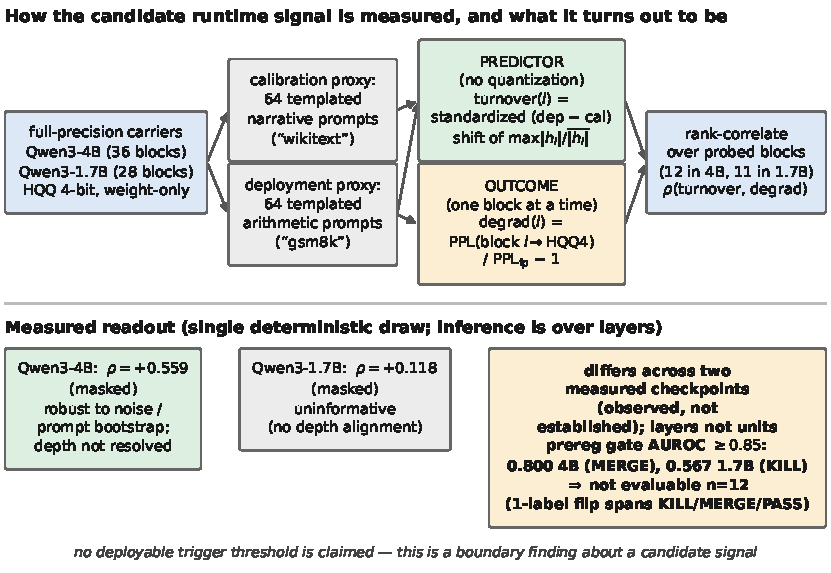
\includegraphics[width=\textwidth]{figures/FIG_pipeline_teaser.pdf}
\caption{What is measured and what comes out. The predictor (green) is computed on the
full-precision model only, from the domain shift of each block's activation-tail ratio; the
outcome (amber) is measured by quantizing exactly one block at a time and re-measuring
deployment-proxy perplexity. The two are then rank-correlated over probed blocks, separately per
carrier. The lower row is the measured readout: a positive but depth-proxied relation on
Qwen3-4B, a null relation on Qwen3-1.7B, and a pre-registered AUROC gate that is measured and not
passed (Limitation~F). Reproduce with
\texttt{python3 experiments/qgate\_tailturnover/r31\_pipeline\_teaser.py}; headline and partial
read at plot time from \texttt{R43\_MASKED\_LADDER.json} (masked primary) and the gate reading from
\texttt{R40\_AUROC\_GATE\_MASKED.json} (corrected pad-masked labels; Limitation~F); figure sha16
\texttt{d5c5a05748f59be5}. This is a programmatic diagram, not a generated image.}
\label{fig:pipeline}
\end{figure}

\section{Introduction}
\label{sec:intro}
Serving a post-training-quantized (PTQ) language model raises a question that calibration-time
accuracy does not answer: can current traffic reveal which quantized blocks will be most damaging?
PTQ reliability can change under calibration drift and input noise \citep{yuan2023benchmarking},
and aggregate quality need not capture all quantization risks \citep{kadadekar2026qualitynotsafety}.
Prior fallback logic uses signals such as numerical overflow \citep{zhang2025int8fallback}, while
other methods remove calibration dependence from the quantizer \citep{son2025nsnquant}. A candidate
runtime trigger must be computable without executing the quantized model and must rank blocks by
their measured quantization damage.

We take one concrete candidate for such a signal and try to falsify it. For each block we measure
the \emph{activation-tail turnover}: how much the ratio of the largest to the mean absolute
activation entering that block shifts when the input distribution moves from the calibration
prompt family to the deployment prompt family, both measured on the full-precision model. As the
outcome we take the true per-block damage: quantize exactly that one block to 4-bit HQQ
\citep{badri2023hqq} and measure the relative increase in deployment perplexity. If the candidate
signal is a usable trigger, these two quantities should agree in rank within a model.
Figure~\ref{fig:pipeline} summarizes the measurement and the answer.

The two measured checkpoints give different point readings, but not an established population
difference: Qwen3-4B \citep{yang2025qwen3} has a positive corrected-label association
($\rho\approx0.56$), whereas Qwen3-1.7B is weak and uncertain ($\rho\approx+0.12$;
Table~\ref{tab:carrier-heterogeneity}, Fig.~\ref{fig:carrier-scatter}). On 4B, turnover is nearly
collinear with depth, and the corrected partial analysis cannot separate them
(\S\ref{sec:results-depth}). Bit-identical replay across three hosts makes the pipeline auditable,
but not independently replicated. We therefore report the candidate signal and its failure modes,
not a trigger threshold or deployment certificate.

\section{What is measured}
\label{sec:method}

\subsection{Predictor: activation-tail turnover, computed without quantization}
\label{sec:method-signal}
Let $h_l(x)$ be the hidden state entering block $l$ of the full-precision model on prompt $x$
(position $l$ of the hidden-state sequence, with position $0$ the embedding output), and define
that block's \emph{tail-mass ratio} on $x$ as the ratio of the largest to the mean absolute
activation over all positions and channels,
\begin{equation}
\mathrm{NTM}_l(x) \;=\; \frac{\max |h_l(x)|}{\overline{|h_l(x)|}} .
\end{equation}
Given a calibration prompt set $D_{\rm cal}$ and a deployment prompt set $D_{\rm dep}$, the
turnover of block $l$ is the standardized shift of this ratio between the two sets,
\begin{equation}
\mathrm{turnover}(l) \;=\;
\frac{\mathbb{E}_{x\in D_{\rm dep}}\!\left[\mathrm{NTM}_l(x)\right]
      - \mathbb{E}_{x\in D_{\rm cal}}\!\left[\mathrm{NTM}_l(x)\right]}
     {\tfrac{1}{2}\left(\mathrm{sd}_{D_{\rm dep}} + \mathrm{sd}_{D_{\rm cal}}\right)} ,
\label{eq:turnover}
\end{equation}
a Cohen's-$d$-style effect size on a per-prompt statistic. Both expectations are taken on the
\emph{full-precision} model: the predictor never sees a quantized weight, which is the property a
runtime trigger needs, and is also why turnover cannot be a mechanical artifact of the outcome.

\subsection{Outcome: true single-block quantization damage}
\label{sec:method-outcome}
For each probed block $l$ we rebuild the model from the full-precision checkpoint, replace every
linear layer inside block $l$ --- the attention and MLP projections, with a fail-closed assertion
that at least six modules were replaced --- by a 4-bit HQQ weight-only layer with group size 64,
leave every other block and the language-model head in full precision, and measure
\begin{equation}
\mathrm{degrad}(l) \;=\;
\frac{\mathrm{PPL}_{D_{\rm dep}}\!\left(M_{l\to\rm HQQ4}\right)}
     {\mathrm{PPL}_{D_{\rm dep}}\!\left(M_{\rm fp}\right)} - 1 .
\label{eq:degrad}
\end{equation}
The quantity of interest is then the rank correlation
$\rho(\mathrm{turnover},\mathrm{degrad})$ over probed blocks of one model: does a block whose
activation tail turns over more also lose more when it, specifically, is quantized?

\subsection{Carriers, domain proxies, probe rule}
\label{sec:method-carriers}
Two carriers of the Qwen3 family \citep{yang2025qwen3} are measured, Qwen3-4B (36 blocks) and
Qwen3-1.7B (28 blocks), in \texttt{bfloat16}, on one \texttt{NVIDIA H20-3e} device per cell. The
probe rule is the fixed index list $[0,1,4,7,12,17,22,27,-4,-3,-2,-1]$ resolved against the block
count and de-duplicated, giving 12 probed blocks on 4B and 11 on 1.7B, i.e.\ early, middle and
the four deepest blocks; the largest probed index therefore pins the block count of each carrier.
The two prompt families are $64$ programmatically templated sentences each, one narrative and one
arithmetic; they are labelled \texttt{wikitext} and \texttt{gsm8k} in the run configuration but
are \emph{not} those corpora, and Limitation~C11 states exactly what they are. Tail statistics use
up to 192 tokens per prompt and perplexity up to 256 tokens, with identical batching for the
full-precision and the single-block-quantized models. Each cell writes one row containing the
probed layer set, per-block turnover, full-precision deployment perplexity and per-block
degradation; the decisive cells are \texttt{4B\_hqq4\_gsm8k} and \texttt{1.7B\_hqq4\_gsm8k} of
one registered run configuration, replayed under a second trial on a different physical host
(run, trial and host identifiers are withheld for double-blind review and given in the anonymous
manifest).

\subsection{Estimators}
\label{sec:method-stat}
Within a carrier we use the Spearman rank correlation over probed blocks. Uncertainty is reported
two ways on purpose --- a Fisher-$z$ interval with $\mathrm{SE}=1/\sqrt{n-3}$ and a percentile
bootstrap resampling blocks --- because at these $n$ the two families disagree about whether zero
is excluded on 4B (Table~\ref{tab:uncertainty-ledger}); the same holds for a two-sided
permutation $p$, which lands on either side of $0.05$ depending on convention. We therefore
condition no claim on a significance threshold, and instead report the point estimate together
with leave-one-block-out (LOO) resampling and the pre-registered drop-block-27 re-check.
Partial rank correlations are computed by residualizing ranks on ranks; they agree with the
closed-form first-order partial correlation to better than $5\times10^{-4}$ on both carriers,
so the depth adjudication in \S\ref{sec:results-depth} does not depend on that implementation
choice. Cross-carrier difference is summarized as $\Delta z$ under Fisher's transform with a
bootstrap interval. An independent re-implementation of the estimators by a separate process
(NumPy rank/tie handling, its own bootstrap and a fixed-seed permutation null with $B{=}20000$)
reproduces $\rho$ on both carriers to the digits printed here: the readout is
estimator-independent, which is a different and weaker property than being data-independent.

\section{Results}
\label{sec:results}

\subsection{The relation is carrier-dependent}
\label{sec:results-main}
Table~\ref{tab:carrier-heterogeneity} gives the readout for both carriers and
Fig.~\ref{fig:carrier-scatter} the underlying per-block scatter; the full Pearson/rank, CI,
LOO and robustness series for the same cells is in Table~\ref{tab:uncertainty-ledger}, Panel~A.
All headline numbers are on the corrected pad-masked degradation (C11); every robustness row is
recomputed on the same masked labels (Table~\ref{tab:uncertainty-ledger}).
On Qwen3-4B the rank (Spearman) correlation between turnover and single-block damage is
positive ($\rho=+0.559$ masked; Table~\ref{tab:carrier-heterogeneity},
Table~\ref{tab:uncertainty-ledger}, Panel~A), and this masked positive relation is robust to
both outcome measurement noise ($P(\rho>0)\approx0.998$ over a noise envelope and a
64-prompt predictor bootstrap; Limitation~C12) and to the depth baseline discussed next.
On Qwen3-1.7B the masked relation is weak and its interval is uninformative
($\rho\approx+0.12$; $P(\rho>0)\approx0.59$), so we report a band classification
(KILL under the pre-registered $|r|<0.15$ rule) rather than a null. The pre-registered rule and
both verdicts are in Appendix Table~\ref{tab:app-gate}; the rank/CI/LOO/robustness series for
both carriers is in Table~\ref{tab:uncertainty-ledger}, Panel~A. Because the pre-registration
defined its PASS/KILL rule over \emph{eight} cells of which only two were run, we report these
two cells as a boundary observation, not as a pass of that rule (Limitation~C12). The
cross-carrier difference points in the sign-flip direction ($\Delta z\approx+0.51$ masked) but,
with two cells and a seed-sensitive interval whose lower edge grazes zero, is observed not
established (Table~\ref{tab:uncertainty-ledger}, Panel~B).

Two honest features of the outcome variable bound how much any of this can mean. First, the
damage is extremely concentrated: in each carrier a single block dominates the readout and the
largest remaining effect is several times smaller, while roughly half the probed blocks land
slightly \emph{below} the full-precision baseline (the concentration rows of
Table~\ref{tab:uncertainty-ledger}, Panel~A). A rank statistic over 11--12 such points is
fragile by construction, which is why we report LOO rather than a single interval; on 4B the
masked LOO range stays positive --- the relation is not the artifact of one block, but it is
carried by a handful of them. Second, the 1.7B cell being uninformative is not a measurement
failure: its dominant block is just as damaged, it simply is not the block whose tail turns
over most.

% P7 QUANT-GATE — Table 1: carrier-dependent heterogeneity + depth-proxy attribution.
% booktabs formal table (MGR R126: each table must be reconstructable — see repro notes below).
% Source data: experiments/qgate_tailturnover/results/fb2_v3/{4B,1.7B}_hqq4_gsm8k.jsonl
%   (run/trial + host identifiers withheld for double-blind review; bit-identical across r-factors and hosts —
%   determinism, effective n=1 across runs per TEACHER r46).
% Repro:  qs training create --config qs/p7_qgate_dec_r1_fb2_v2.yaml   (Trial 1881556)
%         python3 r24_depth_attribution_power.py                        (CPU, depth/LOO/power)
%         python3 r31_paper_numbers.py                                  (CPU, prints every cell)
% Analysis JSON sha16: R24_DEPTH_ATTRIBUTION_POWER.json = fd1bea221759eb4c,
%                      R31_PAPER_NUMBERS.json           = 6c26aced50960e6d.
% R31 change: the 1.7B depth columns, previously left as "--", are filled in from the same
% registered payload; they are what shows that the 1.7B carrier has no depth alignment at all.
\begin{table}[t]
\centering
\caption{Heterogeneity of activation-tail turnover as a predictor of per-layer PTQ degradation
across the two measured checkpoints (HQQ4 weight-only, arithmetic deployment proxy). Writing
$\tau$ for turnover (Eq.~\ref{eq:turnover}), $\delta$ for single-block degradation
(Eq.~\ref{eq:degrad}) on the corrected pad-masked labels (C11) and $d$ for the block index, all
$\rho$ are rank (Spearman) correlations and $\rho(\cdot,\cdot\mid\cdot)$ is a partial rank
correlation, taken over \emph{probed blocks of the same model} --- the unit of analysis is a
layer, not an independent sample (C4, C9). On the masked labels the 4B raw relation is strong
($\rho\approx0.56$) and robust to noise (C12), while $\tau$ is nearly collinear with $d$ and the
masked partials do \emph{not} resolve a depth-proxy attribution (both wide;
\S\ref{sec:results-depth}, C5); on 1.7B the masked relation is weak and its interval
uninformative. The historical unmasked (pad-polluted) values are reported as a superseded
sensitivity row in Table~\ref{tab:uncertainty-ledger}.}
\label{tab:carrier-heterogeneity}
\setlength{\tabcolsep}{6pt}
{\small
\begin{tabular}{lccccccc}
\toprule
Carrier & \shortstack{probed\\blocks} &
$\rho(\tau,\delta)$ & $\rho(d,\delta)$ & $\rho(\tau,d)$ &
$\rho(\tau,\delta\mid d)$ & $\rho(d,\delta\mid\tau)$ &
\shortstack{$\mathrm{PPL}_{\rm fp}$ on\\dep.\ proxy} \\
\midrule
Qwen3-4B   & 12 of 36 & $+0.559$ & $+0.511$ & $+0.909$ & $+0.266$ & $+0.006$ & $18.953$ \\
Qwen3-1.7B & 11 of 28 & $+0.118$ & $+0.091$ & $-0.082$ & $+0.127$ & $+0.102$ & $19.597$ \\
\bottomrule
\end{tabular}
}

\smallskip
\begin{minipage}{\textwidth}
\footnotesize\raggedright
\emph{Reconstruction.} HQQ4 weight-only; calibration proxy $=$ templated narrative prompts,
deployment proxy $=$ templated arithmetic prompts, $n_{\rm cal}=n_{\rm dep}=64$ (C11 states
what these proxies are and are not). $\mathrm{PPL}_{\rm fp}$ is the full-precision
deployment-proxy perplexity, the denominator of every degradation value. Probed-block lists,
analysis JSON sha16s, and the double-blind-suppressed provenance (device / trial / host) are
consolidated in Appendix Table~\ref{tab:app-provenance}. Uncertainty, robustness and power for
these same cells are in Table~\ref{tab:uncertainty-ledger}.
\end{minipage}
\end{table}


\begin{figure}[t]
\centering
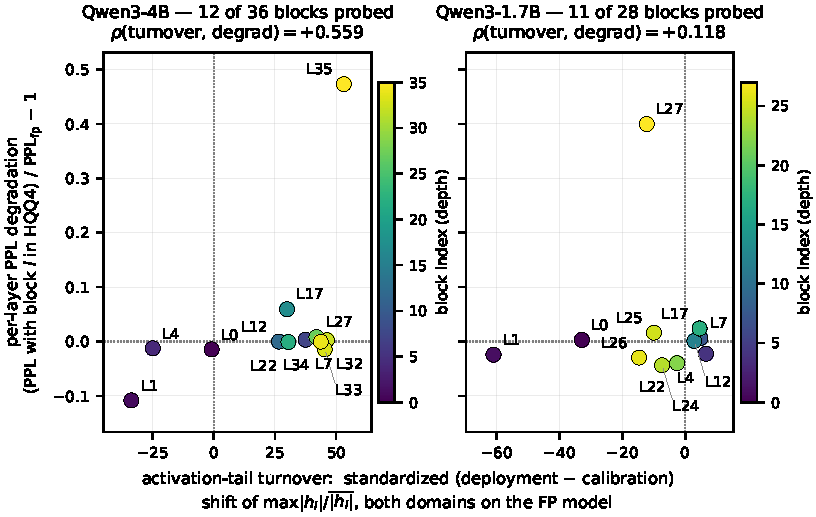
\includegraphics[width=\textwidth]{figures/FIG_carrier_scatter.pdf}
\caption{Per-block activation-tail turnover (Eq.~\ref{eq:turnover}) against single-block PTQ
degradation (Eq.~\ref{eq:degrad}), one point per probed block, coloured by block index. Left:
Qwen3-4B, where turnover and damage both concentrate in the deepest blocks (yellow, upper right)
--- this alignment is the depth proxy quantified in \S\ref{sec:results-depth}. Right:
Qwen3-1.7B, where the deepest probed blocks are spread across the turnover axis and the most
damaged block (27) is not the one with the largest turnover. Axis labels state the estimator
exactly; note that turnover is a deployment-minus-calibration shift measured on the
full-precision model, in pooled standard-deviation units. Reproduce with \texttt{python3
experiments/qgate\_tailturnover/r31\_figure1\_scatter\_v2.py} (0 GPU; plots the masked per-layer
degradation, C11) from the cells of Table~\ref{tab:carrier-heterogeneity}; figure sha16
\texttt{51c69adc4f8f6ee0}.}
\label{fig:carrier-scatter}
\end{figure}

\subsection{Whether the 4B relation is a depth proxy is not resolved}
\label{sec:results-depth}
Turnover and block index (depth) are nearly collinear on 4B ($\rho(\tau,d)\approx0.91$),
which makes the raw positive relation plausibly confounded by depth. On the \emph{unmasked}
(pad-polluted) labels the partial contrast appeared to resolve it: turnover given depth
collapsed toward zero while depth given turnover stayed positive. On the corrected
\emph{masked} labels (the primary analysis) that contrast does \emph{not} reproduce: the masked
partial is $\rho(\tau,\delta\mid d)\approx+0.27$ for turnover given depth and
$\rho(d,\delta\mid\tau)\approx+0.01$ for depth given turnover
(Table~\ref{tab:carrier-heterogeneity}; layer-resampling bootstrap CIs, which are wide, in
Appendix Table~\ref{tab:app-provenance}). Because turnover and depth are so collinear and
$n{=}12$, neither partial is statistically resolved, and the two inferential endpoints point in
different directions: on the AUROC endpoint turnover \emph{exceeds} the depth baseline
($0.800$ vs.\ $0.686$; Limitation~F), while on the masked partials the direction is ambiguous.
We therefore do \emph{not} claim that turnover is a redacted depth proxy, nor that it has
independent predictive value beyond depth: with 11--12 layer-level points we can locate the
confound, not the cause (Limitation~C5). Re-weighting the probed sample to uniform depth
coverage --- removing the probe rule's deliberate deep-decile dominance --- lowers the reported
association ($0.559\to0.401$, R37\_DEPTH\_REWEIGHT\_GATE3;
Limitation~E), and the masked leave-one-block-out range stays positive
($[0.43,0.72]$; the minimum is the masked dominant-block removal, block 35). The 4B headline
is thus positive and robust to noise (L~C12) but its attribution between turnover and depth is
genuinely unresolved. On 1.7B there is little to mediate: depth and damage are essentially
unrelated (Table~\ref{tab:carrier-heterogeneity}), consistent with the weak masked $\rho$. A
mechanistic reading (weight-only damage concentrating where the residual stream has saturated)
is directional only and unsupported by the unresolved partials.

\begin{figure}[t]
\centering
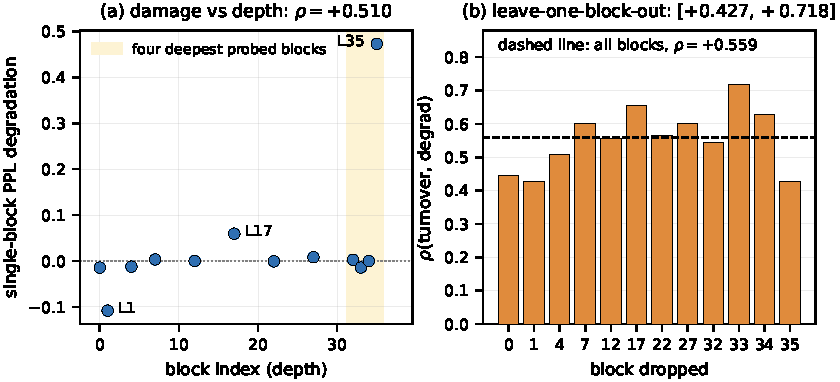
\includegraphics[width=\textwidth]{figures/FIG_depth_attribution.pdf}
\caption{Depth attribution on Qwen3-4B, on the corrected masked labels. (a)~Single-block damage
against block index, with the four deepest probed blocks shaded: the rank relation to depth is
$+0.511$, and the deep zone contains the one block whose quantization is genuinely expensive
(block 35) --- but also blocks that are essentially free, which is why depth is a coarse predictor
rather than a law. (b)~Leave-one-block-out recomputation of $\rho(\mathrm{turnover},\mathrm{degrad})$
(masked): every bar stays positive and the minimum is reached when the dominant block 35 is
dropped ($\rho{=}0.427$), so no single block manufactures the relation; the attribution between
turnover and depth is nevertheless unresolved on the masked partials (C5,
\S\ref{sec:results-depth}). Reproduce with
\texttt{python3 experiments/qgate\_tailturnover/r31\_depth\_attribution\_v2.py}
(0 GPU; plots masked per-layer degradation and asserts the drawn masked LOO range against
\texttt{R43\_MASKED\_LADDER}); figure sha16 \texttt{ec5d743786ec973c}, backing analysis JSON sha16
\texttt{fd1bea221759eb4c}.}
\label{fig:depth-attribution}
\end{figure}

\subsection{Determinism of the readout, and what it is not}
\label{sec:results-determinism}
The decisive cells were executed three times on three different physical hosts and two trials.
The probed layer set, every turnover value, every per-block degradation value and the
full-precision deployment perplexity agree exactly across all three runs
($\max|\Delta| = 0$ in each field; digests in Table~\ref{tab:uncertainty-ledger}). This is worth
stating because it makes the whole readout replayable by a reviewer at the same point, and
because it rules out host- or scheduler-dependent numerical drift. It is equally important what it
does not establish: the three runs are a deterministic replay of a single draw, not independent
samples, so the effective sample across runs is $n_{\rm eff}=1$ and every interval in this paper
is a statement about resampling \emph{layers}, not runs. We consequently never describe this as
cross-run independent replication.

% P7 QUANT-GATE — Table 2: uncertainty / robustness / design-power ledger.
% Panel A is now MASKED-primary (C11): every robustness statistic is recomputed on the
% corrected pad-masked outcome labels. The historical unmasked (pad-polluted) values are
% demoted to a clearly-labelled "superseded" block, per the six-seat panel (P1). Extra rows:
% corrected Fisher-z (Spearman SE 1.06/sqrt(n-3)), masked LOO range, masked drop-top, the
% outcome-noise envelope (R42) and the joint 2D (predictor x outcome) bootstrap (R44).
% Repro: r31_paper_numbers.py (R31_PAPER_NUMBERS.json), r42_noise_envelope.py (R42_NOISE_ENVELOPE.json),
%        r43_masked_ladder.py (R43_MASKED_LADDER.json), r44_turnover_prompt_bootstrap.py (R44_TURNOVER_PROMPT_BOOTSTRAP_{1.7B,4B}.json).
\begin{table}[t]
\centering
\caption{Uncertainty, robustness and design-power ledger (all correlations over \emph{masked}
labels, C11). Panel~A is per carrier; the top block is the masked primary ladder (corrected
Fisher-$z$ uses the Spearman SE $1.06/\sqrt{n-3}$; C5), the middle block adds the
noise-envelope and joint predictor$\times$outcome bootstraps (C12), and the bottom block retains
the superseded unmasked (pad-polluted) values for audit. Panel~B is the cross-carrier
difference. Every interval is over \emph{probed blocks of one model}, so it quantifies sampling
of layers, not of independent runs or models (C4); the \emph{projected} column of Panel~B is
analytic design planning for unexecuted \texttt{zh} cells (C8), not a measured result.}
\label{tab:uncertainty-ledger}
\setlength{\tabcolsep}{5pt}
{\footnotesize
\begin{tabular}{lcc}
\toprule
\multicolumn{3}{l}{\textbf{Panel A --- per-carrier readout (masked primary)}} \\
Quantity (over probed blocks) & Qwen3-4B & Qwen3-1.7B \\
\midrule
$\rho$(turnover, degradation), rank (masked)      & $+0.559$            & $+0.118$ \\
Pearson $r$(turnover, degradation) (masked)       & $+0.463$            & $+0.016$ \\
Fisher-$z$ 95\% CI, Spearman SE (masked)          & $[-0.060,+0.868]$   & $[-0.548,+0.693]$ \\
Bootstrap percentile 95\% CI on $\rho$ (masked)   & $[-0.118,+0.928]$   & $[-0.466,+0.613]$ \\
Permutation $p$ (two-sided, $B{=}20000$) (masked) & $0.031$             & $0.373$ \\
Leave-one-block-out range of $\rho$ (masked)      & $[+0.427,+0.718]$   & $[-0.018,+0.261]$ \\
Drop dominant block, $\rho$ (masked)              & $+0.427$ (block 35) & $+0.261$ (block 27) \\
Largest single-block degradation (masked)         & $+0.473$ (block 35) & $+0.400$ (block 27) \\
Second-largest $|$degradation$|$ (masked)         & $0.108$ (block 1)   & $0.044$ (block 4) \\
\midrule
Outcome-noise envelope $P(\rho{>}0)$ $^{(\mathrm{C12})}$  & $0.9997$   & $0.594$ \\
Envelope $5$th percentile of $\rho$ (noise)       & $0.273$             & $-0.264$ \\
Joint 2D (predictor$\times$outcome) $P(\rho{>}0)$ $^{(\mathrm{C12})}$ & $0.998$ & $0.593$ \\
\midrule
\multicolumn{3}{l}{\emph{Superseded (unmasked, pad-polluted; C11) --- audit only}} \\
$\rho$(turnover, degradation), rank               & $+0.594$            & $-0.109$ \\
Fisher-$z$ 95\% CI (Pearson SE)                   & $[+0.031,+0.871]$   & $[-0.665,+0.525]$ \\
\bottomrule
\end{tabular}
}

\smallskip
\vspace{2pt}
{\footnotesize
\begin{tabular}{lcc}
\toprule
\multicolumn{3}{l}{\textbf{Panel B --- cross-carrier difference and design power (layer-level)}} \\
Quantity & measured (2 cells) & projected (${+}$\texttt{zh}) \\
\midrule
$\Delta z = z(\text{4B}) - z(\text{1.7B})$ (masked) & $+0.513$         & --- \\
$\Delta z$ boot.\ 95\% CI, lower edge over 8 seeds   & $[-0.88,-0.78]$  & --- \\
$\Delta z$ boot.\ 95\% CI, upper edge over 8 seeds   & $[+2.06,+2.17]$  & --- \\
Seeds whose $\Delta z$ CI excludes $0$ (masked)      & $0$ of 8         & --- \\
Fisher SE of $\Delta z$                             & $0.486$          & $0.317$ \\
Registered gate AUROC (masked) $^{(\mathrm{F})}$       & $0.800$          & $0.567$ \\
AUROC, depth baseline (block index) (masked)       & $0.686$          & $0.500$ \\
Noise floor (max within-cell std)                    & $0.013$          & $0.019$ \\
$|\delta| \le$ one noise width (masked)              & $7/12$           & $4/11$ \\
Masked rank-repro vs.\ saved labels $^{(\mathrm{C11})}$ & $0.74$        & $0.88$ \\
Runs / hosts of the decisive readout, $\max|\Delta|$& 3 / 3, $0$       & --- \\
\bottomrule
\end{tabular}
}

\smallskip
\begin{minipage}{\textwidth}
\footnotesize\raggedright
\emph{Reconstruction and method sensitivity.} Masked ladder:
\texttt{r43\_masked\_ladder.py} $\rightarrow$ \texttt{R43\_MASKED\_LADDER.json}; noise envelope:
\texttt{r42\_noise\_envelope.py} $\rightarrow$ \texttt{R42\_NOISE\_ENVELOPE.json}; joint 2D
prompt$\times$outcome bootstrap: \texttt{r44\_turnover\_prompt\_bootstrap.py} $\rightarrow$
\texttt{R44\_TURNOVER\_PROMPT\_BOOTSTRAP\_\{1.7B,4B\}.json} (predictor resampled over the 64
prompts per family, outcome over the measured within-cell spreads, $10^4$ draws each; C12).
Rank/CI/LOO/power series for the same cells: \texttt{r31\_paper\_numbers.py} $\rightarrow$
\texttt{R31\_PAPER\_NUMBERS.json} (sha16 \texttt{6c26aced50960e6d}). The $\Delta z$ seed-envelope
note, partial-$\rho$ bootstrap CIs, pre-registered correlation rule and depth-reweight note are
consolidated in Appendix Table~\ref{tab:app-provenance}; the two pre-registered gate bands and
their verdicts in Appendix Table~\ref{tab:app-gate}. Effective cross-run sample is $1$ (C9);
no interval independently excludes zero on 4B at $n{=}12$ (C5); a single label flip moves the 4B
AUROC across $[0.639,0.889]$ (F, C12).
\end{minipage}
\end{table}


\section{Limitations}
\label{sec:limitations}
The following are binding on how the results above may be read; several of them were fixed as
disclosure requirements before this manuscript was written, and they are the reason the
contribution is stated as a boundary finding.

\begin{itemize}
  \item \textbf{(C4) The unit of analysis is a layer, not an independent sample.} Each carrier
        contributes 12 or 11 probed blocks of one model, and the two carriers share the Qwen3
        architecture. Layers within a model are neither independent nor exchangeable, so every
        interval, partial correlation and power figure here is a layer-level statement carrying a
        pseudo-replication risk, and none of them supports a population-level claim about models.
  \item \textbf{(C5) The confidence-interval family does not resolve zero-exclusion on 4B.}
        Using the conventional Spearman standard error $\mathrm{SE}=1.06/\sqrt{n-3}$ (rather than
        the Pearson form $1/\sqrt{n-3}$ sometimes applied to a rank statistic), the masked 4B
        Fisher-$z$ interval contains zero, as does the percentile bootstrap and the permutation
        $p$ across conventions (Table~\ref{tab:uncertainty-ledger}). No interval independently
        establishes positivity at $n{=}12$; the robustness of the masked 4B direction therefore
        rests on the noise envelope and prompt bootstrap of Limitation~C12, not on any single
        interval. No classification in this paper is conditioned on zero-exclusion or on
        $p<0.05$.
  \item \textbf{(C6) A second analyzer in the repository is configuration-mismatched.} One
        analysis script hard-codes a different results directory and a different cell pair than
        the cells actually executed. The readout here is computed directly with the same
        single-source estimator functions as the primary analyzer, so nothing in this paper
        depends on the mismatched script; we disclose it so that ``the analyzer validated it''
        cannot be inferred.
  \item \textbf{(C7) The pre-registered safety gate's second half ($\ge 30\%$ damage gain) was not
        measured, and the measured artifacts bound it below $30\%$.} The pre-registration's PASS
        condition was an AUROC $\ge 0.85$ trigger \emph{together with} a ${\ge}30\%$ reduction in
        deployment damage over a static clip baseline; the AUROC half is not evaluable at the
        achieved label resolution (Limitation~F). On the damage-gain half, the measured deployment
        FP PPLs ($18.95$ on 4B, $19.60$ on 1.7B) and the measured masked-fallback arms (best
        $16.29$ / $16.95$; \texttt{R41\bk\_GAIN\bk\_BOUND}) give a best relative recovery of
        $\approx 14\%$ / $\approx 13.5\%$, below the $30\%$ gate; reaching $30\%$ would require a
        fallback PPL below the clean (fully-restored) floor. The gain half is therefore
        argued-not-achievable on the measured data, though a definitive negative would need a
        fallback-baseline forward that was not run. Either way this paper makes no claim of having
        passed the registered gate.
  \item \textbf{(F) The registered AUROC half is not evaluable at the achieved label resolution,
        and no trigger is claimed.} The label rule, band definitions, and the AUROC half computed
        on the corrected pad-masked labels are in Appendix Table~\ref{tab:app-gate} (0 GPU;
        \texttt{R40\_AUROC\_GATE\_MASKED}): the 4B AUROC half is $0.800$ (MERGE, not PASS) and the
        1.7B half is $0.567$ (KILL). Because positive is defined as masked degradation $>0$ and over
        half the 4B $|\delta|$ values lie within one measurement-noise width of zero (C12), a
        single label flip moves the 4B AUROC across the KILL/MERGE/PASS span ($[0.639,0.889]$), so
        the achieved $n{=}12$/$11$ label resolution ($\approx 0.03$ AUROC per pair) cannot
        sharpen a $0.15$-wide three-band rule. We therefore report the band reading as a fragility
        record, not as a firm pass-or-fail, and make no deployment-trigger claim on either the
        AUROC or the damage-gain half. On the masked labels the 4B turnover AUROC ($0.800$) sits
        above the trivial depth-baseline AUROC ($0.686$), so the AUROC endpoint does \emph{not}
        independently establish a depth-only reading; the depth interpretation rests on the
        partial correlations of \S\ref{sec:results-depth}, which are themselves unresolved (C5).
  \item \textbf{(C8) The cross-carrier sign difference is not established, and the second-domain
        extension is a decision record, not a result.} The $\Delta z$ bootstrap interval is a
        two-cell statement whose lower edge grazes zero and is unstable under resampling
        ($\Delta z=+0.79$; Table~\ref{tab:uncertainty-ledger}, Panel~B and the seed-envelope
        note below it --- it does not robustly exclude zero --- R35\_DELTA\_Z\_CI\_FIX.json). It
        is therefore observed, not established. Adding the two unexecuted \texttt{zh} cells
        would tighten the Fisher SE and raise the power to detect the observed $|\Delta z|$, but
        even so would remain short of $0.80$ power for the sign flip, which would need a larger
        $|\Delta z|$ (Panel~B and its footnote hold the exact numbers); their real value would be
        testing whether the 4B depth structure reappears in a second domain (projected power
        $>0.8$, Panel~B), not pinning the sign flip. Those cells were not run (estimated
        0.5--1.5 GPU$\cdot$h, pending budget approval); the projected column of
        Table~\ref{tab:uncertainty-ledger} is analytic design planning only.
  \item \textbf{(C9) Bit-identical replay is determinism, not independent replication.} The
        agreement across three hosts and trials demonstrates pipeline determinism with an
        effective cross-run sample of $1$. We write determinism or bit-exactness, never
        cross-run independent replication.
  \item \textbf{(C10) No power analysis backs the primary test; the 4B direction is
        exploratory.} No power analysis was performed for
        $\rho(\mathrm{turnover},\mathrm{degrad})$ itself; the only power numbers available
        (Table~\ref{tab:uncertainty-ledger}, Panel~B) are layer-level design projections for the
        cross-carrier difference and for the depth effect. The 4B positive direction is
        accordingly reported as exploratory, not confirmatory: should any layer-level power
        analysis find the primary test underpowered, that result must be read as an exploratory
        observation and the confirmatory-sounding vocabulary dropped. Because the samples are
        layers, we make no trigger-threshold or deployment-level claim from it under any
        circumstance.
  \item \textbf{(C11) The domain shift is a templated prompt-family shift, and the primary
        analysis is on the corrected pad-masked perplexity.} The families named
        \texttt{wikitext}/\texttt{gsm8k} are not the WikiText-2/GSM8K corpora but 64 single-template
        sentences each (a record-filing and an arithmetic word problem), so the shift is a clean
        low-diversity proxy with reproduction untested on real traffic. The primary analysis is
        computed on masked-perplexity degradation for all 12/11 probed layers
        (\texttt{masked\_from\_log}; pad fraction $0.004$), and the historical unmasked
        (pad-polluted) values are reported only as a superseded sensitivity row. The masked
        headline is $\rho(\mathrm{turnover},\mathrm{damage})=0.559$ on 4B and
        $+0.12$ on 1.7B (Table~\ref{tab:carrier-heterogeneity}); the masked rank-reproduction vs.\
        saved labels is $0.74$ / $0.88$ (Table~\ref{tab:uncertainty-ledger}, Panel~B). Absolute
        perplexities in Table~\ref{tab:carrier-heterogeneity} are not compared with published values.
  \item \textbf{(C12) Effects are of the same order as the outcome's reproduction noise except at
        one or two dominant blocks, and only $2$ of the pre-registered $8$ cells were run.} The
        measured within-cell reproduction spreads of near-zero blocks are milliscale on both
        carriers (five-arm re-measures, \texttt{R39\bk\_NOISE\bk\_RANK\bk\_SYNTHESIS}; noise-floor
        rows in Table~\ref{tab:uncertainty-ledger}, Panel~B), yet over half the 4B probed blocks
        have $|\delta|$ within one maximum noise width of zero. We bound the effect of this on the
        masked headline by a noise envelope (resampling each $\delta$ within its measured
        within-cell spread; \texttt{R42\bk\_NOISE\bk\_ENVELOPE}) and by a predictor bootstrap over
        the 64 prompts per family (\texttt{R44\bk\_TURNOVER\bk\_PROMPT\bk\_BOOTSTRAP}): jointly the
        4B masked $P(\rho>0)\approx 0.998$ ($5$th percentile $\approx 0.22$), whereas the 1.7B
        masked $P(\rho>0)\approx 0.59$ --- the 4B positive relation is robust to both noise sources,
        and the 1.7B cell is uninformative rather than cleanly null. The 4B masked headline still
        rests on one or two dominant blocks: it drops to $0.43$ with the maximum-damage block
        (block 35) removed, which is also the masked leave-one-block-out minimum
        (Table~\ref{tab:uncertainty-ledger}). Separately, the pre-registration defined PASS/KILL over eight cells
        ($2$ carriers $\times$ $2$ quantizers $\times$ $2$ shifts, $\le 6$ GPU$\cdot$h); this
        study ran only two (one HQQ/4-bit quantizer, one shift, Scope), so the registered
        eight-cell rule is not directly evaluable --- we report a two-cell boundary observation
        and claim neither a pass nor a kill of the registered rule.
  \item \textbf{(E) The deep-oversampling probe rule makes the depth structure partly a design
        artifact.} The fixed probe rule $[0,1,4,7,12,17,22,27,-4,-3,-2,-1]$ deliberately places
        four of the twelve probed blocks in the deepest decile, so the depth-graded pile-up of
        \S\ref{sec:results-depth} is in part a consequence of where we chose to probe rather than
        of the underlying per-layer damage distribution alone. We therefore read the depth result
        as a \emph{descriptive} statement about this probe design, not as evidence about the
        uninspected layers, and the inference we draw is limited to the probed blocks. We quantify
        this probe bias on the measured sample by re-weighting each probed block to uniform depth
        coverage (R37\_DEPTH\_REWEIGHT\_GATE3): on 4B the headline becomes
        $\rho(\tau,\delta)=0.401$ when the deep decile ceases to dominate, and the depth
        correlations shrink to the same degree (Table~\ref{tab:uncertainty-ledger}, Panel~A,
        re-weighted rows) --- so the depth proxy survives re-weighting but is partly inflated by
        the probe rule. Re-running the single-block-quantized outcome for the unprobed blocks (a
        depth-uniform or full-layer probe) remains the more expensive step beyond this study's
        budget and is not performed here.
  \item \textbf{Scope.} Two carriers of one family, one quantizer, one bit width, one prompt-shift
        pair, one outcome metric. The 4B positive relation is largely (not fully) a depth proxy, so
        no independent-mechanism claim is made; and since the second carrier is uninformative
        (masked $\rho\approx +0.12$ with a wide interval), we cannot say whether the signal is
        generally weak-but-real rather than absent on other checkpoints.
\end{itemize}

\section{Related work}
\label{sec:related}
\emph{Triggering and fallback.} Runtime-safe quantization triggering has been approached from the
numerical side, with block-level fallback to higher precision when overflow is detected during
INT8 training \citep{zhang2025int8fallback}, and from the quantizer side, by removing the
calibration dependency that creates drift sensitivity \citep{son2025nsnquant}; neither certifies a
deployment-time predictor of per-layer damage, which is what we test. We flag that
\citet{son2025nsnquant} is a \emph{KV-cache} method, whereas this paper quantizes \emph{weights}
only; the comparison is by intent (runtime-safe, calibration-free) rather than by modality.
Reliability studies of PTQ motivate the test itself by showing how much worst-case behaviour moves
under calibration and input shift \citep{yuan2023benchmarking}, and by arguing that task-quality
metrics do not stand in for safety once weights are quantized \citep{kadadekar2026qualitynotsafety}.

\emph{Per-layer sensitivity.} A long line of work treats blocks as individually vulnerable, but
through different mechanisms. GPTQ minimizes second-order error compensation at a \emph{fixed}
width rather than allocating width by sensitivity \citep{frantar2023gptq}; LLM.int8() splits
outlier \emph{columns within a single layer} into high precision rather than ranking layers
\citep{dettmers2022llmint8}; AWQ applies activation-aware \emph{per-channel} scaling without a
layer-level sensitivity score \citep{lin2024awq}; and mixed-precision schemes that do allocate
width by a Hessian- or weight-based per-layer sensitivity score
\citep{dong2019hawq,dettmers2023spqr,kim2024squeezellm} --- which are the natural competitors to
both turnover and our depth baseline --- are computed from an \emph{offline} model/service
analysis, not from a deployment-time \emph{shift} of the input distribution.

\emph{Activation outliers.} The activation-outlier story that motivated activation-aware
quantization has been shown to have a diminishing, calibration-set-dependent effect in modern LLMs
\citep{paglieri2024outliers}; this provides relevant context for our observation. A tail-derived,
calibration-shift-based signal that is positive and depth-confounded on one checkpoint (Qwen3-4B)
and weak-to-uninformative on a smaller sibling (Qwen3-1.7B, masked $\rho=+0.12$ with a wide
interval) is consistent with a diminishing-outlier-effect account, but does not identify that
mechanism. Our per-block framing asks the deployment-time
question both literatures leave open --- can the \emph{shift} of a tail statistic rank per-block
damage? --- and finds that where it appears to, the ranking is largely inherited from block depth,
so any candidate runtime signal must first beat the trivial structural baseline of block index.

\section{Conclusion}
\label{sec:conclusion}
Activation-tail turnover has a positive corrected-label point association with single-block PTQ
damage on Qwen3-4B ($\rho\approx0.56$) and a weak, uninformative association on Qwen3-1.7B
($\rho\approx+0.12$). The cross-checkpoint difference is observed rather than established. On 4B,
turnover is strongly entangled with block depth: reweighting and leave-one-block-out analyses retain
a positive association, but the masked partial correlations do not resolve independent value beyond
depth. Bit-identical replay makes the readout auditable, not independently replicated. These two
checkpoints therefore support an exploratory design lesson---candidate layer-level signals should
be tested against simple structural baselines and across domains---but not a universal fallback
trigger. A second prompt domain and a measured fallback policy are the direct next tests.

\section*{Artifact availability}
Code, per-layer outcome data, and analysis scripts are released: the decisive
\texttt{*\_hqq4\_\allowbreak gsm8k.jsonl} cells and r120 re-runs, the pad-masked recomputation
(\texttt{masked\_\allowbreak from\_\allowbreak log.json}), noise-floor nuisance runs
(\texttt{nuisance\_\allowbreak 4B/1.7B.json}), and the AUROC / robustness tables
(\texttt{R40\_\allowbreak AUROC\_\allowbreak GATE\_\allowbreak MASKED} (canonical, masked labels)
with the historical \texttt{R38\_\allowbreak AUROC\_\allowbreak GATE} and
\texttt{R39\_\allowbreak NOISE\_\allowbreak RANK\_\allowbreak SYNTHESIS}).
Every number cites its \texttt{repro\_command}. Models are the public Qwen3 checkpoints
\citep{yang2025qwen3}; quantization uses HQQ \citep{badri2023hqq}. No generated or synthetic
evidence supports any headline claim.

% The hard gate uses this explicit boundary to count main-text pages. Keep it
% immediately before the bibliography. Do not force a page break: references
% may use the remainder of the final main-text page.
% P5_MAIN_TEXT_END
\label{p5:main-text-end}
\bibliography{refs}
\bibliographystyle{iclr2026_conference}

% Supplementary provenance + pre-registered gate ledger, outside the 9-page main text.
% P7 QUANT-GATE — appendix: provenance + pre-registered gate ledger.
% These tables live AFTER the bibliography, outside the 9-page main text
% (ICLR supplementary policy), and absorb the micro-type provenance footnotes
% of Tables 1/2 and the numeric bands of Limitation F so main-text prose keeps
% only conclusions + table references. Fonts here are >= footnotesize (9pt);
% no \tiny / microfont. All columns are flex X columns; long tokens carry \bk
% (discretionary) break opportunities so no cell can overflow the text block.

\appendix
\section{Provenance and pre-registered gate ledger}
\label{app:provenance}

\subsection{Provenance and reconstruction ledger}
\label{app:provenance-ledger}
Table~\ref{tab:app-provenance} collects the reconstruction and method-sensitivity notes that in
the main text would otherwise sit as dense table footnotes (cf.\
Table~\ref{tab:carrier-heterogeneity} and Table~\ref{tab:uncertainty-ledger}, whose footnotes
here keep only a one-line pointer). All values are reproduced from the registered analysis JSONs
listed in the \emph{source} column.

\begin{table}[H]
\centering
\setlength{\tabcolsep}{4pt}
\caption{Provenance and method-sensitivity ledger. All intervals are over probed blocks of one
model --- the unit of analysis is a layer, not an independent sample (C4).}
\label{tab:app-provenance}
\footnotesize
\begin{tabularx}{\textwidth}{>{\raggedright\arraybackslash}X
 >{\raggedright\arraybackslash}X >{\raggedright\arraybackslash}X
 >{\raggedright\arraybackslash}X}
\toprule
Quantity & Qwen3-4B & Qwen3-1.7B & Source / repro \\
\midrule
Probed blocks & 12 of 36: 0,1,4,7,12,17,22,27,32--35 & 11 of 28: 0,1,4,7,12,17,22,24--27 & fixed probe rule \texttt{0,\bk 1,\bk 4,\bk 7,\bk 12,\bk 17,\bk 22,\bk 27,\bk $-4,-3,-2,-1$} \\
Fisher-$z$ 95\% CI on $\rho$ & $[+0.031,+0.871]$ & $[-0.665,+0.525]$ & \texttt{r31\_\bk paper\_\bk numbers.py} \\
Bootstrap percentile 95\% CI on $\rho$ & $[-0.085,+0.921]$ & $[-0.718,+0.617]$ & \texttt{r31\_\bk paper\_\bk numbers.py} \\
Permutation $p$ (two-sided, $B{=}20000$) & $0.045$ & $0.749$ & \texttt{r31\_\bk paper\_\bk numbers.py} \\
Leave-one-block-out range of $\rho$ & $[+0.473,+0.709]$ & $[-0.273,+0.188]$ & \texttt{r31\_\bk paper\_\bk numbers.py} \\
$\Delta z = z(\text{4B})-z(\text{1.7B})$ lower edge (8 seeds) & $0.794$, $[-0.04,+0.70]$ & --- & \texttt{R35\_\bk DELTA\_\bk Z\_\bk CI\_\bk FIX.json} \\
$\Delta z$ upper edge (8 seeds); seeds excl.\ 0 & $[+0.21,+1.39]$; 7 of 8 & --- & \texttt{r35\_\bk delta\_\bk z\_\bk ci\_\bk fix.py} \\
Fisher SE of $\Delta z$ (projected $+$~\texttt{zh}) & $0.486$ ($0.317$) & --- & \texttt{R35\_\bk DELTA\_\bk Z\_\bk CI\_\bk FIX.json} \\
Power on $|\Delta z|{=}0.794$ (projected) & $0.37$ ($0.71$) & --- & Panel~B \\
Smallest $|\Delta z|$ at 80\% power (proj.) & $1.36$ ($0.89$) & --- & Panel~B \\
Partial-$\rho$ boot.\ 95\% CI, turnover$|$depth & $[-0.49,+0.66]$ & --- & \texttt{R34\_\bk PARTIAL\_\bk CI\_\bk BOOTSTRAP.json} \\
Partial-$\rho$ boot.\ 95\% CI, depth$|$turnover & $[-0.15,+0.88]$ & --- & \texttt{r34\_\bk partial\_\bk ci\_\bk bootstrap.py} \\
Permutation $p$ (layer-resampling) & $0.79$ / $0.18$ & --- & \texttt{r34\_\bk partial\_\bk ci\_\bk bootstrap.py} \\
Depth-reweighted $\rho(\tau,\delta)$ (4B) & $0.401$ & --- & \texttt{R37\_\bk DEPTH\_\bk REWEIGHT\_\bk GATE3} \\
Analysis JSON sha16 & \texttt{6c26aced50960e6d} & same & \texttt{r31\_\bk paper\_\bk numbers.py} \\
Canonical payload digest ($\max|\Delta|{=}0$) & \texttt{04ac77be066fbe87} & \texttt{1b4143950e186756} & sha256 dump, \texttt{sort\_\bk keys} \\
Evidence-ledger audit digest & \texttt{e6325486081538cb} & \texttt{b13c3221d8dedabc} & frozen cross-seat id \\
\bottomrule
\end{tabularx}
\end{table}

\begin{table}[H]
\ContinuedFloat
\centering
\setlength{\tabcolsep}{4pt}
\caption[]{Provenance and method-sensitivity ledger (continued).}
\label{tab:app-provenance-cont}
\footnotesize
\begin{tabularx}{\textwidth}{>{\raggedright\arraybackslash}X
 >{\raggedright\arraybackslash}X >{\raggedright\arraybackslash}X
 >{\raggedright\arraybackslash}X}
\toprule
Quantity & Qwen3-4B & Qwen3-1.7B & Source / repro \\
\midrule
Registered gate AUROC (SAVED pad-polluted labels, r38) & $0.743$ ($p{=}0.10$) / $0.500$ ($p{=}0.54$) & --- & \texttt{r38\_\bk auroc\_\bk gate.py} \\
Registered gate AUROC (MASKED labels, r40) & $0.800$ ($p{=}0.05$) / $0.567$ ($p{=}0.40$) & --- & \texttt{R40\_\bk AUROC\_\bk GATE\_\bk MASKED.json} \\
Depth-baseline AUROC (MASKED labels) & $0.686$ / $0.500$ & --- & \texttt{r40\_\bk auroc\_\bk gate\_\bk masked.py} \\
Sign flips, saved vs.\ masked labels & 4 of 12 & 1 of 11 & \texttt{R40\_\bk AUROC\_\bk GATE\_\bk MASKED.json} \\
\bottomrule
\end{tabularx}
\end{table}

\smallskip
\begin{minipage}{\textwidth}
\footnotesize\raggedright
\emph{Method-sensitivity notes.}
(i)~Bootstrap draws are draw-sensitive at these $n$: a prior archived draw gives
$[-0.099,+0.922]$ on 4B vs.\ $[-0.085,+0.921]$ here --- both contain zero (C5).
(ii)~Two-sided $p$ on 4B is convention-sensitive: $0.042$ asymptotic, $0.0488$ under the
independent-estimator re-implementation, $0.045$ here; no claim is conditioned on $p<0.05$.
(iii)~The three $\Delta z$ rows are the per-seed envelope ($B{=}40000$), i.e.\ a seed-unstable
interval --- why C8 calls the sign difference observed and not established.
(vii)~The partial-$\rho$ CIs span zero, so the partial contrast is directionally consistent but
not statistically resolved. Run config / device / trial / host identifiers are withheld for
double-blind review and given in the supplementary manifest.
\end{minipage}

\subsection{Pre-registered gate ledger}
\label{app:gate-ledger}
Table~\ref{tab:app-gate} is the decision record for the two pre-registered safety flags; it
replaces in-prose repeats of the bands in Limitation~F and \S\ref{sec:results-main}.

\begin{table}[H]
\centering
\setlength{\tabcolsep}{4pt}
\caption{Pre-registered gate ledger: band rules, measured values, and verdict (computed 0 GPU
from the registered cells on the \emph{corrected pad-masked} labels; depth baseline is the
trivial block-index predictor). The AUROC half is computed under masked labels as disclosed in
Limitation~F; the raw pad-polluted label readout is reported in
Table~\ref{tab:app-provenance} for the label-source record, and the full three-label-set table
is \texttt{R40\_AUROC\_GATE\_MASKED.json}.}
\label{tab:app-gate}
\footnotesize
\begin{tabularx}{\textwidth}{>{\raggedright\arraybackslash}X
 >{\raggedright\arraybackslash}X >{\raggedright\arraybackslash}X
 >{\raggedright\arraybackslash}X}
\toprule
Gate / rule & Band definition & 4B measured / 1.7B measured (masked labels) & Verdict \\
\midrule
Pearson $r$ PASS/KILL (raw relation) & PASS $\ge 0.3$; MERGE $0.15\le r<0.3$; KILL $<0.15$ & $+0.490$ / $+0.021$ & PASS / KILL (2 cells only, C12) \\
Registered AUROC gate & PASS: AUROC $\ge 0.85$ \emph{and} $\ge 30\%$ gain; MERGE $0.7\text{--}0.85$; KILL $<0.7$ & $0.800$ ($5/12$; perm.\ $p{=}0.05$) / $0.567$ ($6/11$; $p{=}0.40$) & MERGE / KILL; NOT passed; band fragile (F, C12) \\
Damage-gain half (NOT evaluated; no fallback forward) & PASS requires $\ge 30\%$ damage reduction & FP PPL $18.95/19.60$; clean reference $16.29/16.95$ ($\approx14\%/13.5\%$ feasibility bound) & Feasibility-bound below target; no fallback measured (C7) \\
\bottomrule
\end{tabularx}

\smallskip
\begin{minipage}{\textwidth}
\footnotesize\raggedright
\emph{Notes.} Values are the AUROC half over probed blocks, labels positive iff masked
degradation $>0$ (\texttt{R40\_AUROC\_GATE\_MASKED.json}). At the corrected masked labels the
trivial depth-baseline AUROC is $0.686$ (4B) / $0.500$ (1.7B) --- i.e.\ the depth baseline does
\emph{not} beat the turnover AUROC on either carrier, correcting Limitation~F.
The band verdict is fragile: a single label flip moves the 4B AUROC to anywhere in
$[0.639,0.889]$, spanning KILL/MERGE/PASS, and the 4B mask label count rests on one near-zero
layer (C12). The gate's damage-gain half ($\ge 30\%$) needs a fallback-baseline simulation and
was not run (C7). Both rules were defined over \emph{eight} cells of which only two were run
(C12), so both classifications are boundary observations, not passes or kills of the rules.
\end{minipage}
\end{table}


\end{document}
